\documentclass[11pt,letterpaper,twosided]{memoir}
\usepackage{georgebook}
\usepackage{draftwatermark}
\usepackage{bera}

\author{George Flanagin}
\date{\today}

\chapterstyle{madsen}

%\SetWatermarkText{Work in Process}
\SetWatermarkText{}
%\SetWatermarkText{QAnon}
\SetWatermarkFontSize{6cm}
\SetWatermarkAngle{55}
\SetWatermarkColor[gray]{0.98}

\setlength{\parskip}{0.8em}
\setlength{\parindent}{0.8em}

\title{A Field Guide to ETL Planning and Implementation\\
\large for Managers, Business Analysts, and Programmers}
\author{George Flanagin\\
\normalsize\lit{gflanagin@richmond.edu}~\lit{me@georgeflanagin.com}}
\date{\today}

\setsecnumdepth{subsection}
\maxsecnumdepth{subsection}
\settocdepth{subsection}
\maxtocdepth{subsection}

\semiisopage
\checkandfixthelayout

\begin{document}
\sloppybottom
\maketitle
\begin{abstract}
This guide covers issues related to the design, selection,
and implementation of an ETL system. It is based in part on the
author's experiences at \UR, a private university in Virginia, USA.
The issues are discussed in terms of how they affect a company
with a modest size technology support organization, and a large
number of small software systems, each with its own handful of 
data integrations. 
\end{abstract}
\newpage
\tableofcontents
\listoffigures
\newpage
\renewcommand\thelinenumber{\color{red}\arabic{linenumber}}
\pagewiselinenumbers
\modulolinenumbers[3]

\frontmatter
%%%%%%%%%%%%%%%%%%%%%%%%%%%%%%%%%%%%%%%%%%%%%%%%%%%%%%%%%%%%%%%%%%%
\chapter{Foreword: Who is the reader?}
If your organization exchanges data between systems, internally or
externally, then you have an ETL system. It may not meet your needs;
it may not be what you want; but you have an existing system. As
a reader, you are probably interested in changing it and improving
it, but it is important to remember that if your organization is
exchanging data then \emph{there is an existing system}, and it is
best to understand it well before you start changing things.

ETL is not a new term, and of late \emph{data integrations} is a
popular noun-phrase that has replaced the verbs \emph{extract,
transform}, and \emph{load}.  There are as many sets of vocabulary as there
are vendors and consultants combined, and the vocabulary is often
related to some larger methodology that is being promoted, as well.
In this pamphlet, we will do our best to speak of the ETL tasks
without tying the conversation to any current or past point of view.

This guide should be read by everyone connected with
ETL so that everyone involved has a common base-level understanding
of ETL activities, and everyone on the team speaks the same language,
using the same words of description to thereby avoid misunderstandings.
Common vocabulary saves time and money.

In this guide,
the first use of a \emph{term of art} appears in italics, and is
defined in a nearby footnote.\footnote{\emph{Term of Art} is a
phrase that has a specific meaning within the scope of this document.}
If you read the guide ``cover to cover,'' this will serve you well. 
If you forget what a term means, there is a glossary at the end.

\section{A few words on style}

As the author, I have tried to maintain consistency with the intent
to improve understanding. For example, \emph{data} is always used
as a plural noun, and this has allowed me to use \emph{datum} as
the singular. My choice prevents endless uses of tiring phrases like
\emph{piece of data}.

Conversations about pronouns are all the rage in 2020 as I write
the first edition of this pamphlet. I find that reading \emph{his
or her} breaks the flow of the narrative, and the singular \emph{they}
still sounds plural to many readers' ears. Regardless of concerns
about gender and number, prounouns have a tendency to make the text
confusing, and in this document I have tried to minimize their use,
and instead spell out the job function of the person I am discussing
in the text.

I have also opted for a first and second person delivery, so I will
speak in the text directly to \emph{you} about \emph{your} processes,
and when there is a collective enterprise \emph{we} will speak of
\emph{us} and \emph{our} work. This reads more normally and less
formally.

My co-workers have told me that I have an idiosyncratic choice of
words. I am sure it is true. There are a few words that do not appear 
in this document, for example, this sentence is the only one that
contains \emph{utilize}. The word \emph{use} is correct, and it is
short and widely understood. There is one exclamation point in
this document, which I hope also implies that you will not find
anything in here to be surprising or astonishing. The text is not
trendy or clever, just informative.

In fact, 
the point of this guide is to transfer my knowledge to you, to help
you be successful and reduce your ETL costs and the consequent 
suffering associated with poorly informed choices.

\begin{flushright}George Flanagin\\\today\end{flushright}

\mainmatter
%%%%%%%%%%%%%%%%%%%%%%%%%%%%%%%%%%%%%%%%%%%%%%%%%%%%%%%%%%%%%%%%%
\chapter{Design}

I originally wrote the chapter title as ``Requirements of an
ETL system,'' but something about the formality of the text
put me off. Because an ETL system joins other systems, the 
requirements are as much about the boundaries of the system as
they are about what is \emph{in} the ETL system.

Figure~\ref{fig:mindmap} is taken from the collective discussion
at \UR that preceded all our decisions about formalizing and 
choosing an ETL system. Many of the requirements are generic
in the sense that your organizaiton will be considering them
for every Tier 1 business system that you buy or build.

\begin{figure}
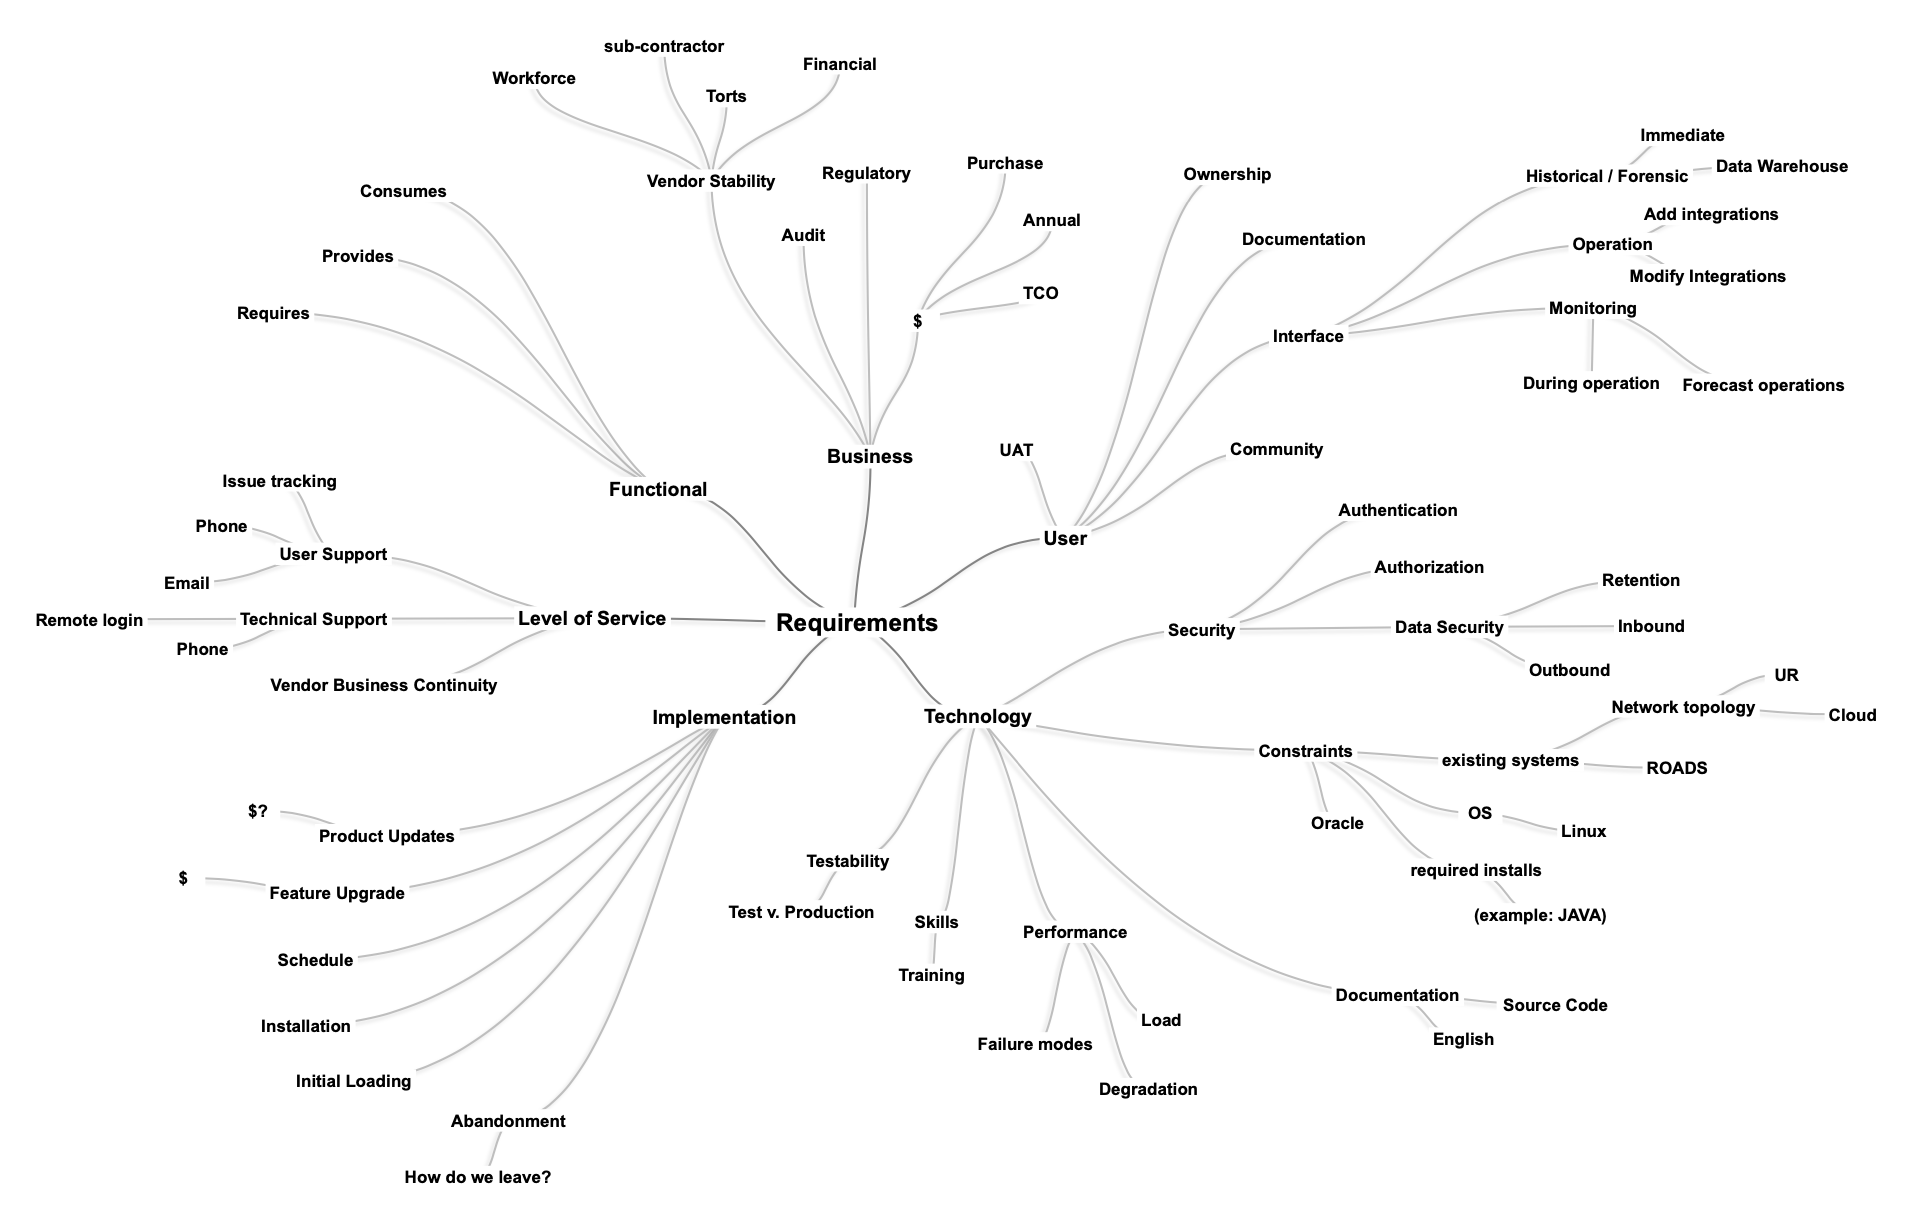
\includegraphics[width=0.95\textwidth]{mindmap.png}
\caption{Mind-map of ETL requirements from \UR}
\label{fig:mindmap}
\end{figure}

\section{Why do we need to design ETL systems?}

Starting with design may seem unusual, but it is definitely the
place to start.  Whether you build or buy, you must design the
functions of your ETL system. This is true whether you are buying
an OTS product, customizing one, or going from scratch. This chapter
is about how to perform this task; without this step you are flying
blind.

The time spent on design creates policies about how your systems
interact.  In turn, the policies eliminate the need to decide the
specifics of each ETL operation case by case; instead, the project
manager consults the policies and acts accordingly. The reduction
in maintenance cost is significant. In Chapter~\ref{chap:staffing}
there is a discussion of ETL staffing, and the costs will be lower
if all the ETL operations are self-similar and consistent, the
desired result of following a policy.

ETL systems have one very large scale property that constrains
acceptable designs. Using the conventional and current vocabulary,
let us call each element of the ETL system an \emph{integration}.\footnote{
There is no universally accepted definition of a [data] integration.
In this guide, I define an integration as something that can be
launched and run separately from other integrations, and that 
on its own can be said to succeed or fail. As an example, there
might be a weekly integration that collects a list of employees
who are paying for supplemental dental insurance, and transfers
it to the insurance provider. It does not interact with other
operations, and it either succeeds or fails without the need
to examine other data transfers.}

\section{Index cards}

I first encountered the use of index cards as a project management
tool in a workshop at The University of Canberra, intriguingly
titled \emph{Low-rez Prototyping}.  Rather than using PowerPoint
or Keynote, and concerning himself with style and color, the
instructor wrote on large, plain white index cards with a black
marker, and stuck them to the wall with thumbtacks. The lesson of
efficiency combined with expediency and low cost has not changed
in value over the years.

A collection of index cards with your design elements, one per card
can be used in any number of ways. They can be sorted many times,
and they can be divided among team members who are assigned
responsibility for defining the subject of the card.

In terms of systems and subsystems, I have had good luck with the
following facts and properies on the cards. I use the term
\emph{subsystem}\footnote{A subsystem is possibly a standalone
``thing,'' with the property that it can be started, stoped, bought,
sold, replaced, \etc, without having to alter other subsystems. A
system is a collection of one or more subsystems that inter-operate.
The important characteristic of this arbitrary definition is that
it is testable. Also, note its similarity to the definition of 
\emph{integration}.} rather than \emph{thing} or \emph{item}, because
subsystem and system are terms of art.

\begin{description}
\item[Name:] The proper noun that you will use for this subsystem.
Good names are [1] easy to spell, [2] hard to forget, and [3] not
in use anywhere else in your organization. If it is possible to
have the names of related parts suggest the familial nature of their
relationship, then do so. As an example, you might name all the
financial systems after world currencies so that they are known as
Lira, Mark, Drachma, and Peso. But Cookie, Cracker, Toast, and
Breadstick are just as memorable.

The abstract names have a definite security advantage, as well. If
you are loose of lip and having a glass of wine in a semi-public
place, you are less likely to reveal specific information about
company internals if you say unflattering things about Toast and
Butter than if you refer to the product by its better known name.

\item[Type:] There will be more about this topic below. Important 
factors in the type information are facts that are answers to questions
like ``Did you buy it?'' and ``Is it a physical object?''

\item[Description:] A very rough idea of what it is. This description
is ideally just enough for everyone who reads it to have the
\emph{Aha!} moment and be able to distinguish this subsystem from
anything similar enough to be occasionally confused with it.

\item[Owner:] Owner is not an ideal noun because it can be ambiguous.
The owner of a subsystem is a \emph{person}, not a group of people,
who is the final arbitrator of whether or not the system is working
as it should. Clearly, an owner must understand the \emph{purpose}
of the subsystem to make this judgment, even if all the \emph{functions}
are not understood.  \footnote{Purpose and function are used
interchangeably by some writers.  Within this guide, they are not.
A purpose serves an end goal, and a function is simply an action
of some kind. Asset management is a purpose, whereas producing a
financial report of the assets is a function.}

\item[Contact info:] Again, the contact info should identify and
be associated with a human being. ``The help desk'' is not a suitable
piece of the contact info. Seek out direct phone numbers, and the
email addresses of specific people, especially in the case of the
owner.


\end{description}

\section{Endpoints}

\emph{Endpoint} is the term we will use for the sources, destinations,
and intermediate rest-stops for data as it moves through your
enterprise.  Motion and transformation take place between the
endpoints, and the key concept of an endpoint is that it very likely
has some unique constraints that involve the format of your data.

It is essential to give your endpoints (and many other things)
names, and each one should have at least one index card associated
with it. Again, well known names prevent endless recurrences of
phrases like ``the system over at the recreation center,'' and the
resulting ambiguity about exactly what is in that system.

\section{Boundaries}

Without well defined boundaries, your ETL system will not work at
all. As the data move between endpoints, they cross over the boundary
into the ETL system, and assuming they do not get lost, they again
cross the boundary in the outward direction. 

You can draw the boundaries wherever it suits your business needs.
At \UR, we made a collection of decisions about what was inside and
outside of the ETL system. These specific decisions worked
well for us; they might not be the right ones for you, but you
must have a definition or two bad consequences will follow. 
You may have duplicated effort within the ETL system, or you
may find that you have falsely assumed which system will have the
shown here are presented in Figure~\ref{fig:boundaries} only as an
example to help you think through the process of defining the
boundaries in your own systems and subsystems.

\begin{figure}[ht]
\begin{center}
\small
\begin{tabular}{lp{0.7\textwidth}}
\toprule
\textbf{Category}&\textbf{Boundary consideration}\\
\midrule
embedded info&The ETL system only knows things by their names. The ETL
system does not know about database schemas, the mechanics of Oracle or 
MSSQL. Instead it only knows to get \emph{everything} in a database 
view because it only knows the name of the view.\\

mutability&The ETL system does not inspect the data moving through
it.  If a change is to be applied (encryption, creating a CSV file,
\etc), the change must be applied to the entire collection of data
uniformly.\\

integrity&The ETL system runs each E-T-L route through it in a separate
process. Doing so prevents data leakage, and ensures that if an operation
crashes, other simultaneous operations will be unaffected.\\ 

orientation&As a design principle, the ETL system reaches out to retrieve
files, rather than having them delivered. Similarly, it delivers files to
foreign endpoints rather than leaving them at an internal collection point
for pickup.\\

one entrance&Each E-T-L route only takes information from a single named
source. This implies that the ETL system does not combine data from
several sources; it has no knowledge of how to do so.\\

notifications&The ETL system does not send email beyond subject-line-only
acknowledgements; it is up to the receiving
endpoint to provide detailed information if that is a desired action.\\

no validation&The ETL system assumes that the data it receives is 
correct, and it does not do proofreading of the data. This is similar
to the way manufacturing systems work; components are assumed to have
been inspected before they are delivered.\\

\bottomrule
\end{tabular}
\caption{Example ETL boundaries}
\label{fig:boundaries}
\end{center}
\end{figure}

The benefits of boundaries are much like the advice offered by
Robert Frost that ``good fences make good neighbors.'' The strong
boundaries remove the need to discuss whether or not leaving files
on a \emph{DMZ}\footnote{DMZ refers to an area of your network that
is simultaneously accessible to processes inside and outside your
network.} endpoint is a good idea, or whether the ETL system should
send text messages.

Reality, being obnoxious at times, forced us to make \emph{minor}
adjustments to our rules. For example, we had a case of a vendor
producing files that were in the format of an encrypted file, but
they were not encrypted at all.  Our decryption software did not
care (following its own principle of not doing receiving inspection),
and no error was reported. After we discovered the problem, we added
a small plugin to the ETL system to check that encrypted files were
encrypted and signed.

\section{Design for the common cases}

A few years ago, I visited a family member in metropolitan Atlanta.
He took me for a drive in his new AMG modified Mercedes-Benz, V8
engine, stick shift, and almost immediately we were comfortably
lodged in traffic between lesser vehicles on all sides. He did not
keep the car very long because he discovered that it was not designed
for the common case of being stuck in traffic, although as a passenger
I must admit the zero-to-twenty performance was outstanding.

Within my industry (higher education), there are three families of
ETL operations that are reasonably common.

\begin{enumerate}
\item Regularly scheduled data transfers. Regularly scheduled covers
a lot of ground, and it can range from an hourly transfer of information
about new customers or changes in inventory, to monthly taxation
data. The idiosyncrasies of the calendar mean that \emph{two days
before the last working day of the month} is paradoxically both regular
and irregular.

\item \emph{Ad hoc} transfers. I have found that these are generally
corrective actions of some type. The integration may require re-execution
because the destination was offline when the transfer was attempted,
or because some change that has been made to the data source must
be urgently reflected in the destination system.

\item Event driven data transfers. No ETL system can be aware of every
event in the IT environment, but any reasonable ETL system should 
be able to monitor and respond to at least a few well defined events. 
The appearance of a new file and a new message in a queue are examples
of useful events.

\end{enumerate}

There are a few additional ETL operations that do not involve
the ETL system. For example, if you are migrating a business system
from the local data center to a cloud host, you may need to unload
the entire database and recreate it in the new environment; extract
and load without the transformation. We do not generally see this
action as within the reasonable expections of the ETL system.

\section{Defining the meaning of success}
\label{sec:success}

Strangely, this is an important design goal. Consider a data
integration that begins with a database query that creates a delta
or difference result set. Only things that have changed since the
last execution are reported. Suppose nothing has changed? An empty
set is just as much a successful result as a few hundred items.

Now consider an import of daily credit card charges. In any company 
larger than a few people, it is unusual to go a day without some
credit card activity. In a sense, your system ``expects'' there to
be a daily supply of data. Finding nothing is at least a good
reason to inspect the result.

However, this cannot be a rigid policy. Many data integrations
are checked more often than data is presumed to be available in
the interest of keeping the systems up-to-date. 

\subsection{Syntactic success}

\subsection{Semantic success}

\section{A requirements checklist}

The use of a checklist prevents errors of omission, and errors
of omission are the most common design gaffe with ETL systems. The
following is a quick list, and it includes many topics that apply
to any Tier 1 business system.

\begin{description}
\item[Business:] The type of business you are in affects many of
the decisions you will make about an ETL system.

\begin{enumerate}
\item Costs, ranging across initial purchase, annual licensing, and
TCO (Total Cost of Ownership).
\item Regulatory constraints if you are in a highly regulated business.
\item Auditing, including security and other IT-type audits.
\end{enumerate}

\item[Vendor stability:] Assuming you have decided to buy a system
rather than build it, vendor stability is the most often overlooked 
consideration. Many customers do not question a vendor's business stability
although it is straightforward to gather much of the data.

\begin{enumerate}
\item Be alert to whether the vendor has sub-contractors of its own.
This is an additional source of instability.

\item Financial records for public corporations are easy to obtain
from authoritative sources. 
\end{enumerate}
\end{description}


%%%%%%%%%%%%%%%%%%%%%%%%%%%%%%%%%%%%%%%%%%%%%%%%%%%%%%%%%%%%%%%%%
\chapter{Build \emph{v}. Buy}

There is no complete ETL system.

%%%%%%%%%%%%%%%%%%%%%%%%%%%%%%%%%%%%%%%%%%%%%%%%%%%%%%%%%%%%%%%%%
\chapter{ETL Staff Requirements}
\label{chap:staffing}

\section{Political considerations}

ETL operations lie on the irregular border between information 
technology interal operations and the (internal or external) 
customer's world. 

\section{Implementation skills}

\section{Operational skills}

%%%%%%%%%%%%%%%%%%%%%%%%%%%%%%%%%%%%%%%%%%%%%%%%%%%%%%%%%%%%%%%%%
\chapter{Common and Uncommon Problems in ETL Systems}

ETL systems have as many problems as they have moving parts. To the
best of my knowledge, there is no way to reduce their frequency
because many of them have their origins outside the ETL system, and
merely happen to be discovered when a data transfer or manipulation
is attempted.

\section{What is an acceptable level of reliability?}

In 2020, \UR's ETL system executed a little less than one thousand
transfer operations per day, with anywhere between zero and ten
``files'' transfered per operation. That's a lot to go wrong, and
na{\"i}vely it is not far off to say that with 1000 operations per
day, an error rate of $0.1\%$ means something is broken every day.
This phenomenon has been likened to the original Space Shuttle that
contained around 100,000 custom parts and systems, each of which
was highly reliable on its own. Yet the interaction and the number
of parts led to many launch delays, and at least two spectacular
failures.

Let's consider some ways to improve reliability in an ETL system
by using it effectively.

\subsection{Following the order of operations}

The name \emph{ETL} gives a clue where to start. The pattern of 
operations is what it appears to be --- first extract, then tranform,
then load. From the perspective of the designer, whether in-house or
the vendor's designer, it may be tempting to offer options and
flexibility. Perhaps only could load some data into a database,
execute a stored procedure involving the new data, and then pull 
a report based on it?

The appeal of doing so is easy to understand. Directness is usually
desireable, and flexibility is often pitched alongside the buzzwords
\emph{scriptable}, \emph{configurable}, and \emph{customizable}, 
what Peter DeGrace called the abilities in his 1990 book \emph{Wicked
Problems; Righteous Solutions}.

As a rule, if the loading takes place before the extraction, then the
loading is not a part of the same ETL operation as the extraction. 
The advice is sometimes difficult to follow. 

Suppose you are currently using a fancy shell script for each
integration. Regardless of your opinion about the elegance or
usefulness of the shell's language, there is no doubt that it is
flexible. Having seen integration shell scripts as long as 1400
lines to load information about courses and students into the
Blackboard\CircleR\thinspace system, I can attest to their abilities
to tie themselves into incomprehensible and unmaintainable knots.
It is quite tempting to transport the shell script's logic into the
ETL system as a direct translation, and depending on your ETL system,
it might be doable, but in doing so you break the ETL symmetry.

\subsection{Separation of duties}

If your business systems are at all old, you may have database
procedures that are the workhorses of the organization. At the time
they were constructed, the adaptation of SQL into a procedural language
could have been your organization's main axe. Compiled procedures,
stored in the database, might produce a file format that exactly 
matches the destination's requirements, and you are most likely to
find this behavior with integrations that deal with regulated 
industries like banking and insurance.

Any reasonable business has change controls. 

\section{Extraction}

\subsection{Abstracted sources of data}

This topic can also be called \emph{loose coupling} of the ETL
system. Using databases as an example source of data, A list of 
things you should never do is shown in Figure~\ref{fig:donts}.

\begin{figure}
\begin{framed}
\begin{quote}
No matter how tempting, do not:

\small
\begin{itemize}

\item Allow the ETL system to exploit the identity of the database.
The database should have a \emph{name}, and that's all. The fact it
is an Oracle database or a MySQL database should remain invisible
to the ETL system. Even the names of database VIEWs should employ 
synonyms to preserve the anonymity of the underlying schema or
other container. 

\item Reveal the details of the SELECT statement to the ETL system.
Instead, all the SQL logic should be contained in a database VIEW
that is known only by its name to the ETL system. The ETL system
should limit itself to \lit{SELECT * FROM myview}.

\item Tweak the contents of a VIEW after the SELECT. In other words,
when the VIEW has a bug, fix it in the VIEW and avoid embedding
knowledge in the ETL system with statements like \lit{SELECT * FROM
myview WHERE some\_column is NOT NULL}.  That may seem obvious, but
it will be tempting to make data repairs in the ETL system because
it will likely have looser controls than the systems of record
containing the data.

\end{itemize}
\end{quote}
\caption{Don'ts of data extraction}
\label{fig:donts}
\end{framed}
\end{figure}

\subsection{Choosing a representation for the extracted data}

I have hammered the nail representing the need to follow standards 
hard in the preceding pages, and the principle of having a single
way of doing things applies here, as well.

\section{Transformation}

\subsection{The null transformation}

From the design of the earliest processors, the need for the null 
operation, or \lit{NOP} as it was often written, was recognized by
everyone involved in the design of programming languages. 

\subsection{Flavors of CSV}

If the recipient of CSV data is an Excel\CircleR\thinspace spreadsheet,
the choices made during the production of the CSV make little 
difference. Often, the CSV file is delivered to an older system, and
these older systems are brittle.\footnote{Brittle: my intent is to
convey that, like glass, the systems are useful, and strong when they are intact.
However, their fault tolerance is poor, and when they fail it is
always catastrophic.}

\subsection{XML}

\subsection{Encryption}

There is no doubt that in 2020, encryption is not much more widely
practiced by IT professionals than it was in 2010 or 2000.
Complicating this void in professional backing is the fact
that ETL operations are often turned over to people who are not IT
professionals at all, and consequently do not even possess even a
\emph{poor} understanding of the many issues around encryption.
If you choose not to encrypt delivered files, and if you choose to
receive unencrypted files, the risk is high and the amount of time
saved is trivially small compared with the effort to repair and
recover from a small data leak.

If you lean toward sanity, the management of all the encryption
keys is within your ETL system. The idea that the encryption software
itself (WinPGP, gpg, GnuPG, \etc) is an attractive fantasy ---
impossible because only the ETL system knows the association of
each vendor's key with the identity of one or more ETL operations
for that vendor.\footnote{I limited this discussion to vendors
because there is not a good case for transfers of encrypted data
within the organization. Doing so would be what security pioneer
Gene Spafford described as using an armored car to move a bag of
cash between two park benches. Source: \emph{Wired}, 25 November
2002.}

\subsection{File formats: Linux/UNIX v. Windows v. Mac}

Particularly when the delivery endpoint is a Windows machine, or
the file is destined to find itself being read on a Windows platform,
the file must have the correct kind of end-of-line marker. On Linux,
the common practice in professional software is to analyze the first
couple of kilobytes of the file when it is believed that the file
is organized by lines, and make an almost always correct guess about
the way the end of lines are marked.\footnote{On the operating
systems whose names end with ``\lit{X}'' a single linefeed character
is used. On Windows, the end of line is marked by a carriage return
followed by a linefeed.}

Outside of Asia, the world largely represents characters with 
the \lit{UTF-8} encoding scheme. Large books have been written
about character encoding schemes, and some of them have even been
read. 

\section{Loading and Delivery}

\section{ETL Hygiene}

It is tempting to believe that a sigh of relief is appropriate the
moment that an data integration successfully delivers the files its
target. 

\subsection{Cleaning up detritus}


\subsection{Confirmations}

In Section~\ref{sec:success}, I mentioned the importance of a 
definition of success with an ETL operation. Where practical, it is 
good to attempt confirmation of success. 


\appendix
\chapter{Glossary}

\end{document}

































